%
% File: chap01.tex
% Author: Victor F. Brena-Medina
% Description: Introduction chapter where the biology goes.
%
\let\textcircled=\pgftextcircled
\chapter*{Introduction}
\label{chap:intro}
\addstarredchapter{Introduction}
\markboth{Introduction}{}
\section*{CONTEXT}
\initial{S}\lipsum[2] 

\par \lipsum[2]

\begin{figure}[!h]
	\centering
    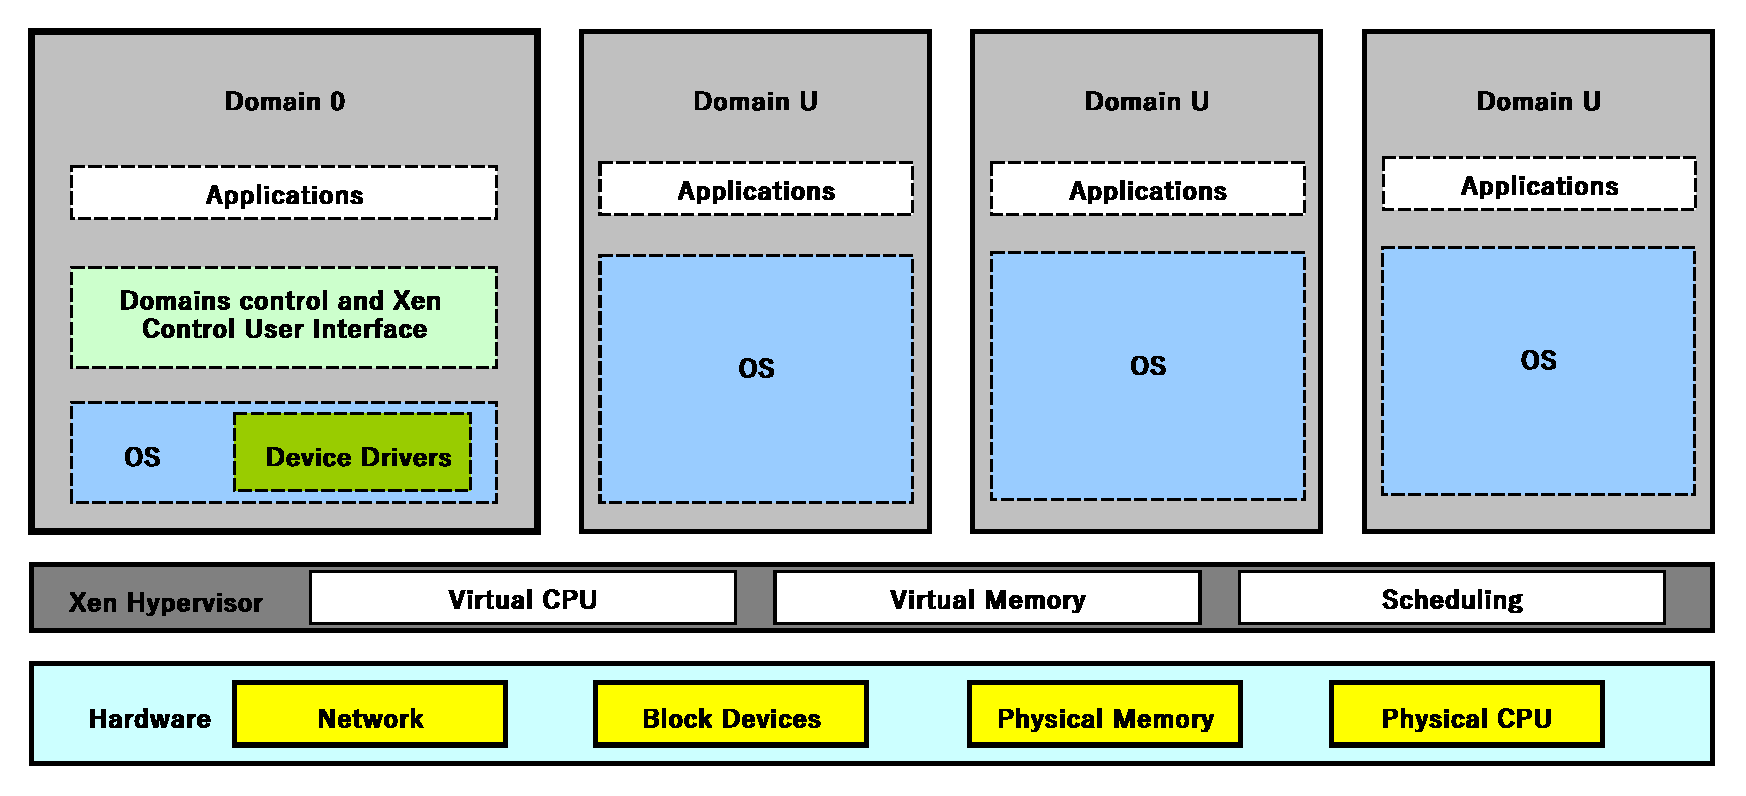
\includegraphics[width=\linewidth]{fig01/xen_simple.pdf}
    \caption{Simplified Xen Architecture}
    \label{fig:arch_simple_xen}
\end{figure}

\section*{PROBLEMATIC}

\lipsum[2]

\begin{bidentidad}{Question}
\begin{itemize}
    \centering How should resources be allocated to the dom0 and organised in a \\ \acrshort{numa} architecture ? 
\end{itemize}
\end{bidentidad}

\section*{OBJECTIVES}
The main goal of this work is to establish a \textbf{resource allocation strategy for the dom0} that will take into consideration the two fundamental questions mentioned above. Our resource allocation strategy should enable: 

\begin{enumerate}
    \item the dom0 to have exactly the amount of resources it needs at every moment,
    \item the dom0 processes that work on behalf of a virtual machine use the resources of this virtual machine and 
    \item those processes must be executed as close as possible to the virtual machine for which they work.
\end{enumerate}

To achieve this, we explored the issues associated with these two questions, analyzed the limitation of previous solutions addressed to this problem and compared our resulting model to the existing solutions on a series of \glspl{bench}s well thought out for the problem.

\section*{ROAD MAP}
The rest of the document is structured as follows: 

\begin{itemize}
    \item \textbf{Background} in which we enrich our vocabulary and present some mechanisms in the Xen architecture for a better understanding of the work and what follows;
    \item \textbf{Problem statement and assessment} where we discuss about the questions raised in the problematic and prove it is relevant;
    
\end{itemize} 
